\documentclass[a4paper,12pt]{article}
\usepackage[a4paper, total={180mm, 272mm}]{geometry}

\usepackage{fontspec}
\setmainfont[Path=fonts/, Extension=.ttf]{ipaexm}

\setlength\parindent{3.5em}
\setlength\parskip{0em}
\renewcommand{\baselinestretch}{1.247}

\usepackage{eepic}
\usepackage{xcolor}

\usepackage{graphicx}
\graphicspath{{images/}}

\begin{document}

\thispagestyle{empty}

\Large
\noindent \\
HSV Noise Ino\medskip
\par
\normalsize
Add pixel noise to the Hue, Saturation, Brightness, and Alpha.\par
The addition of noise adjustment to the cell picture, has been developed\par
for the purpose of adapting the picture of the background.\\
\par
The Alpha channel will determine the strength of the noise. Therefore,\par
smooth edges will remain smooth.\par
The strength of the Alpha channel itself will also affect noise, check the value.\\
\par
When you check the results, please do not use the sub-camera.\par
This is because in the sub-camera the range of the input image is different,\par
the noise pattern will change.\\
\\
-{-}- \ Inputs \ -{-}-\\
Source\par
Connect the image to process.\\
Reference\par
Connect the reference image to put the strength of the effect into each Pixel.\\
\\
-{-}- \ Settings \ -{-}-\\
Hue\par
Specify the strength of the noise for the color (Hue).\par
Pixel value (8 or 16bits) specified as a value from 1 to 0.\par
Minimum value is 0, maximum value is 1.\par
It does not apply the noise to the color (Hue) when the value is 0.\par
The default value is 0.025.\\
\\
Saturation\par
Specify the strength of the noise for the chroma (Saturation).\par
Pixel value (8 or 16bits) specified as a value from 1 to 0.\par
Minimum value is 0, maximum value is 1.\par
It does not apply the noise for the chroma (Saturation) when the value is 0.\par
The default value is 0.0.\\
\\
Value\par
Specify the strength of the noise for the brightness (Value).\par
Pixel value (8 or 16bits) specified as a value from 1 to 0.\par
Minimum value is 0, maximum value is 1.\par
It does not apply the noise to the brightness (Lightness) when the value is 0.\par
The default value is 0.035.

\newpage

\thispagestyle{empty}

\ \vspace{-0.2em}
\par
\noindent Alpha\par
Specify the strength of the noise for the Alpha channel.\par
Pixel value (8 or 16bits) specified as a value from 1 to 0.\par
Minimum value is 0, maximum value is 1.\par
It does not apply the noise to the Alpha channel when the value is 0.\par
The default value is 0.0.\\
\\
Seed\par
The value of the order to determine the random noise pattern of the image.\par
Specify an integer value greater than or equal to 0.\par
If this value is the same, it will reproduce the same pattern.\par
It will be a different pattern If you add the noise with a different value.\par
The default value is 1.\\
\\
NBlur\par
It blurs the noise component, reduces the dot  impression.\par
Minimum value is 0, maximum value is 1.\par
Because it is calculated only in pixels adjacent to the dot,\par
it will feel like a very light blur.\par
When the blur value is not 0, it will take the average of the pixels adjacent\par
to each other up to a value of 1.0.\par
The default value is 1.\\
\\
Limits\par
The chroma (Saturation), brightness (Value), opacity (Alpha),\par
adjustment to effect the end value (in the vicinity of 0 to 1).\par
Applying the noise at 0 or near 1, will appear below 1 or more than the value of 0,\par
so it can not be expressed, because the values are each truncated to 0 or 1.\par
It is effective to compensate for the truncation.\par
-{-}> \textquotedbl End value of Noise effect adjustment \ \ Figure 1 \ \ comparison\textquotedbl \ reference\par
-{-}> \textquotedbl End value of Noise effect adjustment \ \ Figure 2 \ \ description\textquotedbl \ reference\\
\par
\noindent \ \ \, Effective\par
Determines the strength of this effect (Limits).\par
It has no effect if the value is 0. Effect a table using a value greater than 0\par
A value of 1 will have the strongest effect.\par
The default value is 0.\\
\par
\noindent \ \ \, Center\par
Determines the center of the effect.\par
Noise range deviation, the effect of the reduction of the noise width, most strongly\par
at the portion of 0 to 1 of the end value, will have no effect in the center.

\newpage

\thispagestyle{empty}

\ \vspace{-0.2em}
\par
Position the center value without this effect.\par
The value must be between 0 and 1.\par
If the value is 0, it will have no effect on a Pixel with a value of 0.\par
If the value is 1, it will have no effect on a Pixel with a value of 1.\par
The default Center value is 0.5.\\
\par
\noindent \ \ \, Type\par
Select from the options of the Type of the effect.\par
If you select \textquotedbl Keep Noise\textquotedbl , it maintains the (overall) noise width shifting of the\par
noise range, the contrast of the entire image will shrink.\par
If you select \textquotedbl Keep Contrast\textquotedbl , it maintains the contrast to reduce the noise width\par
only at the end.\par
The default setting is \textquotedbl Keep Noise\textquotedbl .\\
\\
Premultiplied\par
When ON, RGB is already set to Premultiply\par
(The value of Alpha channel is multiplied in advance RGB channels)\par
and processes as an image.\par
At that time, and added to the Alpha processing, you may not get the correct image.\par
The default setting is ON.\\
\\
Reference\par
Choose how Reference image values put the strength of the effect into each Pixel.\par
An image is connected to the \textquotedbl Reference\textquotedbl \ of the input,\par
Choose from Red/Green/Blue/Alpha/Luminance/Nothing.\par
Choose Nothing when you do not want this effect, it will turn off the connection.\par
The default setting is Red.

\newpage

\thispagestyle{empty}

\ \vspace{1.5em}
\par
\noindent \hskip 2.2em Figure 1 Noise effect comparison of the values\\[0.4em]
\par
\scriptsize
\noindent \hskip 3.4em Original\par
\noindent \hskip 3.4em Effective Zero\par
\noindent \hskip 3.4em Keep Noise\par
\noindent \hskip 3.4em Keep Contrast

\large
\noindent \begin{picture}(0,0)
\put(55.5,-6.5){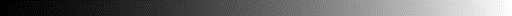
\includegraphics[width=29.6em, height=1em]{HSVNoiseInoNoiseEffectOriginal}}
\put(55.5,-22.5){
\includegraphics[width=29.6em, height=1em]{HSVNoiseInoNoiseEffectEffectiveZero}}
\put(55.5,-38.5){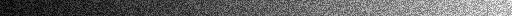
\includegraphics[width=29.6em, height=1em]{HSVNoiseInoNoiseEffectKeepNoise}}
\put(55.5,-54.5){
\includegraphics[width=29.6em, height=1em]{HSVNoiseInoNoiseEffectKeepContrast}}
\linethickness{0.01em}
\put(126,64){\line(-1,0){56}}
\put(126,53){\line(-1,0){14}}
\put(126,41){\line(-1,0){42}}
\put(126,29.5){\line(-1,0){28}}
\put(126,15){\line(-1,0){93}}
\put(126,64){\line(0,-1){49}}
\put(33,15){\line(0,-1){58}}
\put(33,0){\line(1,0){14}}
\put(47,0){\line(-3,2){6}}
\put(47,0){\line(-3,-2){6}}
\put(33,-14){\line(1,0){14}}
\put(47,-14){\line(-3,2){6}}
\put(47,-14){\line(-3,-2){6}}
\put(33,-28){\line(1,0){14}}
\put(47,-28){\line(-3,2){6}}
\put(47,-28){\line(-3,-2){6}}
\put(33,-43){\line(1,0){14}}
\put(47,-43){\line(-3,2){6}}
\put(47,-43){\line(-3,-2){6}}
\end{picture}\\[3.6em]

\normalsize
\noindent \hskip 2.2em Figure 2 Noise range change illustration of the values\\[0.5em]
\par
\footnotesize
\noindent \hskip 2.65em Effective Zero \ \ The value of the noise is cut (default)

\large
\noindent \begin{picture}(0,0)
\linethickness{0.01em}
\put(54.5,-37){\line(0,1){8}}
\put(54.5,-37){\line(-2,3){3}}
\put(54.5,-37){\line(2,3){3}}
\put(482,-37){\line(0,1){8}}
\put(482,-37){\line(-2,3){3}}
\put(482,-37){\line(2,3){3}}
\put(54.5,-58){\line(0,1){6}}
\put(482,-58){\line(0,1){6}}

\put(27,-45.5){\line(1,0){56}}
\put(27,-45.5){\line(3,2){6}}
\put(27,-45.5){\line(3,-2){6}}
\put(83,-45.5){\line(-3,2){6}}
\put(83,-45.5){\line(-3,-2){6}}

\put(255,-45.5){\line(1,0){56}}
\put(255,-45.5){\line(3,2){6}}
\put(255,-45.5){\line(3,-2){6}}
\put(311,-45.5){\line(-3,2){6}}
\put(311,-45.5){\line(-3,-2){6}}

\put(455,-45.5){\line(1,0){56}}
\put(455,-45.5){\line(3,2){6}}
\put(455,-45.5){\line(3,-2){6}}
\put(511,-45.5){\line(-3,2){6}}
\put(511,-45.5){\line(-3,-2){6}}

\put(61,-67){\line(1,0){15}}
\put(61,-67){\line(3,2){6}}
\put(61,-67){\line(3,-2){6}}
\put(52,-70){\scriptsize{0}}
\put(78,-74){\footnotesize{0 or less of the noise value is limited to 0}}

\put(471,-67){\line(-1,0){15}}
\put(471,-67){\line(-3,2){6}}
\put(471,-67){\line(-3,-2){6}}
\put(476,-70){\scriptsize{1.0}}
\put(312,-74){\footnotesize{1 or more noise is limited to 1}}

\linethickness{0.2em}
\put(54.5,-38){\line(1,0){428}}
\linethickness{2.8em}
\put(49,-1.5){\line(1,0){439}}
\linethickness{2.75em}
\color{lightgray}
\put(45.5,-1.5){\line(1,0){438}}
\put(51,-0.5){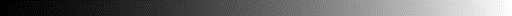
\includegraphics[width=29.55em, height=1em]{HSVNoiseInoNoiseEffectOriginal}}
\put(51,-16.5){
\includegraphics[width=29.55em, height=1em]{HSVNoiseInoNoiseEffectEffectiveZero}}
\end{picture}\\[5.7em]

\footnotesize
\noindent \hskip 2.65em Keep Noise \ \ Shift to maintain the noise. Contrast is reduced. It shifts the overall noise position

\large
\noindent \begin{picture}(0,0)
\linethickness{0.01em}
\put(255,-45.5){\line(1,0){56}}
\put(255,-45.5){\line(3,2){6}}
\put(255,-45.5){\line(3,-2){6}}
\put(311,-45.5){\line(-3,2){6}}
\put(311,-45.5){\line(-3,-2){6}}

\put(158,-60){\line(0,1){8}}
\put(158,-60){\line(-2,3){3}}
\put(158,-60){\line(2,3){3}}
\put(400,-60){\line(0,1){8}}
\put(400,-60){\line(-2,3){3}}
\put(400,-60){\line(2,3){3}}

\put(144,-68.5){\line(1,0){56}}
\put(144,-68.5){\line(3,2){6}}
\put(144,-68.5){\line(3,-2){6}}
\put(200,-68.5){\line(-3,2){6}}
\put(200,-68.5){\line(-3,-2){6}}

\put(357,-68.5){\line(1,0){56}}
\put(357,-68.5){\line(3,2){6}}
\put(357,-68.5){\line(3,-2){6}}
\put(413,-68.5){\line(-3,2){6}}
\put(413,-68.5){\line(-3,-2){6}}

\put(107,-83){\line(0,1){8}}
\put(107,-83){\line(-2,3){3}}
\put(107,-83){\line(2,3){3}}
\put(442,-83){\line(0,1){8}}
\put(442,-83){\line(-2,3){3}}
\put(442,-83){\line(2,3){3}}

\put(102,-91.5){\line(1,0){56}}
\put(102,-91.5){\line(3,2){6}}
\put(102,-91.5){\line(3,-2){6}}
\put(158,-91.5){\line(-3,2){6}}
\put(158,-91.5){\line(-3,-2){6}}

\put(392,-91.5){\line(1,0){56}}
\put(392,-91.5){\line(3,2){6}}
\put(392,-91.5){\line(3,-2){6}}
\put(448,-91.5){\line(-3,2){6}}
\put(448,-91.5){\line(-3,-2){6}}

\put(58,-106){\line(0,1){8}}
\put(58,-106){\line(-2,3){3}}
\put(58,-106){\line(2,3){3}}
\put(478.5,-106){\line(0,1){8}}
\put(478.5,-106){\line(-2,3){3}}
\put(478.5,-106){\line(2,3){3}}

\put(55,-114.5){\line(1,0){56}}
\put(55,-114.5){\line(3,2){6}}
\put(55,-114.5){\line(3,-2){6}}
\put(111,-114.5){\line(-3,2){6}}
\put(111,-114.5){\line(-3,-2){6}}

\put(427,-114.5){\line(1,0){56}}
\put(427,-114.5){\line(3,2){6}}
\put(427,-114.5){\line(3,-2){6}}
\put(483,-114.5){\line(-3,2){6}}
\put(483,-114.5){\line(-3,-2){6}}

\put(283,-106){\line(0,1){54}}
\put(267,-123){\scriptsize{separate}}

\linethickness{0.2em}
\put(54.5,-38){\line(1,0){428}}
\put(54.5,-61){\line(1,0){428}}
\put(54.5,-84){\line(1,0){428}}
\put(54.5,-107){\line(1,0){428}}
\linethickness{2.8em}
\put(49,-1.5){\line(1,0){439}}
\linethickness{2.75em}
\color{lightgray}
\put(45.5,-1.5){\line(1,0){438}}
\put(51,-0.5){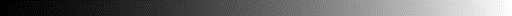
\includegraphics[width=29.55em, height=1em]{HSVNoiseInoNoiseEffectOriginal}}
\put(51,-16.5){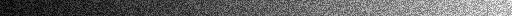
\includegraphics[width=29.55em, height=1em]{HSVNoiseInoNoiseEffectKeepNoise}}
\end{picture}\\[9.3em]

\footnotesize
\noindent \hskip 2.65em Keep Contrast \ \ Reduce the noise width. Maintain the contrast. Noise width is reduced only at the end

\large
\noindent \begin{picture}(0,0)
\linethickness{0.01em}
\put(255,-45.5){\line(1,0){56}}
\put(255,-45.5){\line(3,2){6}}
\put(255,-45.5){\line(3,-2){6}}
\put(311,-45.5){\line(-3,2){6}}
\put(311,-45.5){\line(-3,-2){6}}

\put(86,-60){\line(0,1){8}}
\put(86,-60){\line(-2,3){3}}
\put(86,-60){\line(2,3){3}}
\put(450,-60){\line(0,1){8}}
\put(450,-60){\line(-2,3){3}}
\put(450,-60){\line(2,3){3}}

\put(58,-68.5){\line(1,0){56}}
\put(58,-68.5){\line(3,2){6}}
\put(58,-68.5){\line(3,-2){6}}
\put(114,-68.5){\line(-3,2){6}}
\put(114,-68.5){\line(-3,-2){6}}

\put(423,-68.5){\line(1,0){56}}
\put(423,-68.5){\line(3,2){6}}
\put(423,-68.5){\line(3,-2){6}}
\put(479,-68.5){\line(-3,2){6}}
\put(479,-68.5){\line(-3,-2){6}}

\put(70,-83){\line(0,1){8}}
\put(70,-83){\line(-2,3){3}}
\put(70,-83){\line(2,3){3}}
\put(468,-83){\line(0,1){8}}
\put(468,-83){\line(-2,3){3}}
\put(468,-83){\line(2,3){3}}

\put(55,-91.5){\line(1,0){28}}
\put(55,-91.5){\line(3,2){6}}
\put(55,-91.5){\line(3,-2){6}}
\put(83,-91.5){\line(-3,2){6}}
\put(83,-91.5){\line(-3,-2){6}}

\put(454,-91.5){\line(1,0){28}}
\put(454,-91.5){\line(3,2){6}}
\put(454,-91.5){\line(3,-2){6}}
\put(482,-91.5){\line(-3,2){6}}
\put(482,-91.5){\line(-3,-2){6}}

\put(61,-106){\line(0,1){8}}
\put(61,-106){\line(-2,3){3}}
\put(61,-106){\line(2,3){3}}
\put(476.5,-106){\line(0,1){8}}
\put(476.5,-106){\line(-2,3){3}}
\put(476.5,-106){\line(2,3){3}}

\put(55,-114.5){\line(1,0){12}}
\put(55,-114.5){\line(3,2){6}}
\put(55,-114.5){\line(3,-2){6}}
\put(67,-114.5){\line(-3,2){6}}
\put(67,-114.5){\line(-3,-2){6}}

\put(471,-114.5){\line(1,0){12}}
\put(471,-114.5){\line(3,2){6}}
\put(471,-114.5){\line(3,-2){6}}
\put(483,-114.5){\line(-3,2){6}}
\put(483,-114.5){\line(-3,-2){6}}

\put(283,-106){\line(0,1){54}}
\put(267,-123){\scriptsize{separate}}

\linethickness{0.2em}
\put(54.5,-38){\line(1,0){428}}
\put(54.5,-61){\line(1,0){428}}
\put(54.5,-84){\line(1,0){428}}
\put(54.5,-107){\line(1,0){428}}
\linethickness{2.8em}
\put(49,-1.5){\line(1,0){439}}
\linethickness{2.75em}
\color{lightgray}
\put(45.5,-1.5){\line(1,0){438}}
\put(51,-0.5){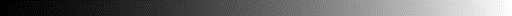
\includegraphics[width=29.55em, height=1em]{HSVNoiseInoNoiseEffectOriginal}}
\put(51,-16.5){
\includegraphics[width=29.55em, height=1em]{HSVNoiseInoNoiseEffectKeepContrast}}
\end{picture}

\end{document}